\subsection{Simulation environment and topologies}\label{sec:imp-sumo}
All control runs in SUMO with TraCI. Six topologies span a
regular-synthetic to irregular-real axis along which \S\ref{ch:results}
finds the largest differences, without isolating which property carries
them: two synthetic grids (3$\times$3, 4$\times$4), a Bloomsbury grid from
OpenStreetMap, the Euston A501 corridor and its peak-hour variant, and the
Old Street complex junction. Euston's AADF-derived demand carries the
A501's measured DfT vehicle mix but an assumed hourly profile, the
peak-hour variant rescaled to the measured DfT peak-hour magnitude. Old
Street's nine signals include a single five-arm, seventeen-movement
junction, demand-calibrated after default random demand gridlocked it, as
were the Bloomsbury grid and Euston peak-hour corridor
(\S\ref{sec:res-calib}). Only Euston's demand magnitude is measured, the
other two real maps being randomTrips draws (\S\ref{sec:dis-threats}).
Figure~\ref{fig:sumo-gui} shows the Bloomsbury network under the
calibrated demand.

\begin{figure}[t]
\centering
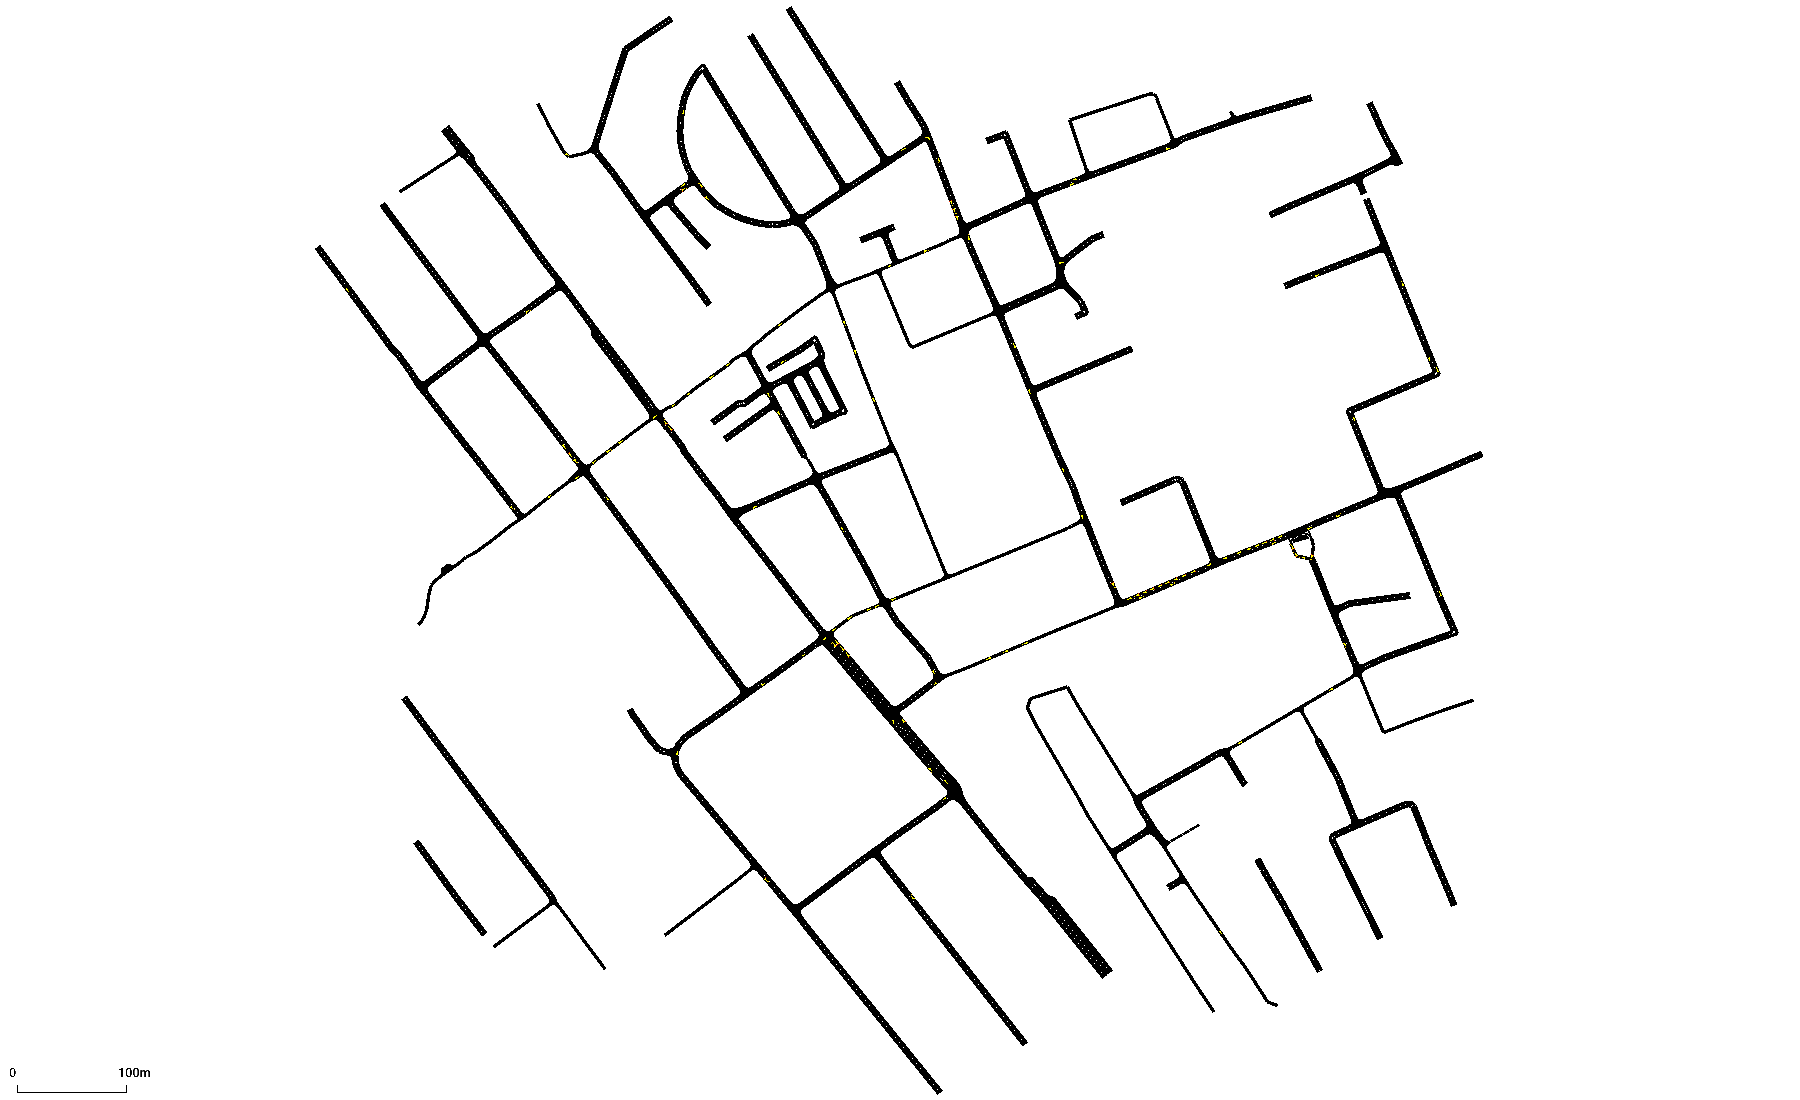
\includegraphics[width=\columnwidth]{figures/bloomsbury-sumo-gui.png}
\caption{The Bloomsbury network in SUMO at $t{=}420$\,s under the
calibrated 40\% demand (seed 1): nine signalised junctions extracted from
OpenStreetMap, 112 vehicles in motion.}
\label{fig:sumo-gui}
\end{figure}
